\chapter{Kiểm thử hệ thống}
\subsection{Tổng quan về kiểm thử}

Mục đích của kiểm thử trong hệ thống: Đảm bảo rằng các tính năng hoạt động đúng, hệ thống không có lỗi và có thể chịu được tải trong quá trình sử dụng thực tế.

Loại kiểm thử thực hiện:
\begin{itemize}
	\item \textbf{Kiểm thử chức năng:} Đảm bảo các chức năng của hệ thống hoạt động đúng
	\item \textbf{Kiểm thử hiệu suất:} Đảm bảo hệ thống có thể xử lý nhiều yêu cầu đồng thời
	\item \textbf{Kiểm thử bảo mật:} Đảm bảo hệ thống bảo vệ tốt các dữ liệu người dùng
	\item \textbf{Kiểm thử tích hợp:} Kiểm tra sự hoạt động đồng bộ của các module
	\item \textbf{Kiểm thử hồi quy:} Đảm bảo những thay đổi mới không làm hỏng các tính năng cũ
\end{itemize}


\subsection{Mô tả chung về các kịch bản kiểm thử}

Mỗi kịch bản kiểm thử được tổ chức và theo dõi theo bảng sau đây. Các mục chính trong mỗi kịch bản kiểm thử bao gồm:
\begin{itemize}
	\item \textbf{TEST SCENARIO:} Tên kịch bản kiểm thử
	\item \textbf{Screen name/Function name:} Tên màn hình hoặc tên chức năng cần kiểm thử
	\item \textbf{Test case code:} Mã số của test case
	\item \textbf{Number of passed test cases (P):} Số lượng test case đã thành công
	\item \textbf{Number of failed test cases (F):} Số lượng test case không thành công
	\item \textbf{Number of test cases under pending (PE):} Số lượng test case đang chờ xử lý
	\item \textbf{Number of unexecuted test cases:} Số lượng test case chưa được thực hiện
	\item \textbf{Total number of test cases:} Tổng số test case cần kiểm thử
\end{itemize}

\subsubsection{Cấu trúc của một kịch bản kiểm thử}

\begin{itemize}
	\item \textbf{Test case code:} Mã của test case, giúp phân biệt các test case khác nhau
	\item \textbf{Testing Purpose:} Mục đích của việc kiểm thử
	\item \textbf{Steps:} Các bước thực hiện kiểm thử
	\item \textbf{Expected outcome:} Kết quả mong đợi sau khi thực hiện các bước kiểm thử
	\item \textbf{Browser compatibility testing:} Kiểm tra tính tương thích với các trình duyệt phổ biến
	\item \textbf{Test status report:} Báo cáo tình trạng của các lần kiểm thử
\end{itemize}

\subsubsection{Ví dụ về một kịch bản kiểm thử trong bảng Excel}
\begin{figure}[H]
	\centering
	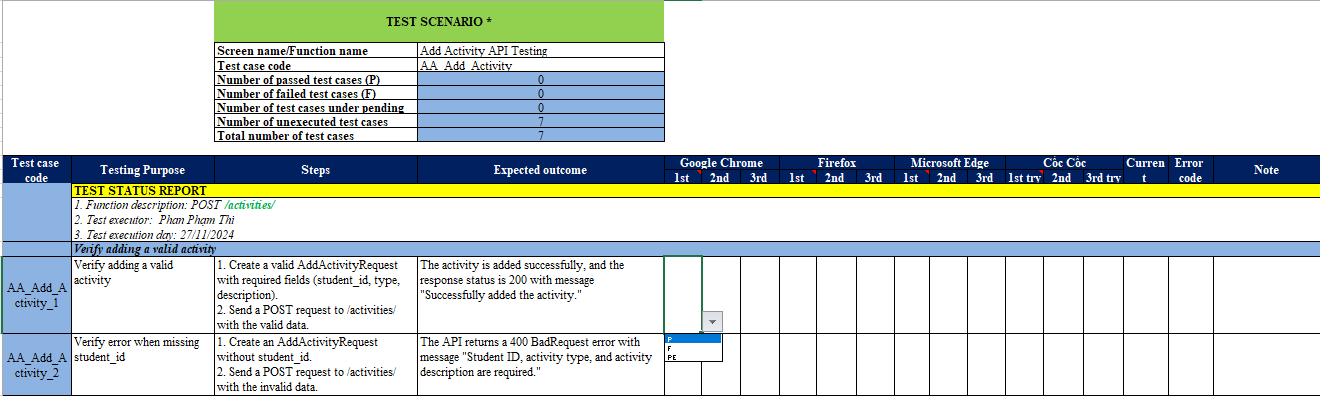
\includegraphics[scale=0.5]{Images/Implement/testScenario.png}
	\caption{Ví dụ về một kịch bản kiểm thử}
\end{figure}
\subsubsection{Mục tiêu của các kịch bản kiểm thử}
\begin{itemize}
	\item \textbf{Kiểm thử chức năng}: Đảm bảo các API hoạt động đúng với các yêu cầu và dữ liệu đầu vào hợp lệ hoặc không hợp lệ.
	\item \textbf{Kiểm thử tương thích trình duyệt}: Đảm bảo hệ thống hoạt động ổn định trên các trình duyệt phổ biến.
	\item \textbf{Kiểm thử độ tin cậy}: Kiểm tra xem các API có thể xử lý được các tình huống thực tế và đưa ra kết quả chính xác.
\end{itemize}

\section{Các API cần kiểm thử}
Các APIs được kiểm thử sẽ là các APIs có liên quan đến các chức năng chính của hệ thống như:
\begin{itemize}
	\item Sinh ra lộ trình học tập cho sinh viên
	\item Theo dõi tiến độ học tập của sinh viên
	\item Sinh ra bài tập quiz tự động cho sinh viên
	\item Sinh ra bài tập lập trình tự động cho sinh viên
	\item Đánh giá tiến độ học tập của sinh viên
\end{itemize}
\subsection{Phân tích chi tiết các kịch bản kiểm thử}

\subsubsection{Kiểm thử API Tạo Lộ Trình Học Tập}
\begin{figure}[H]
	\centering
	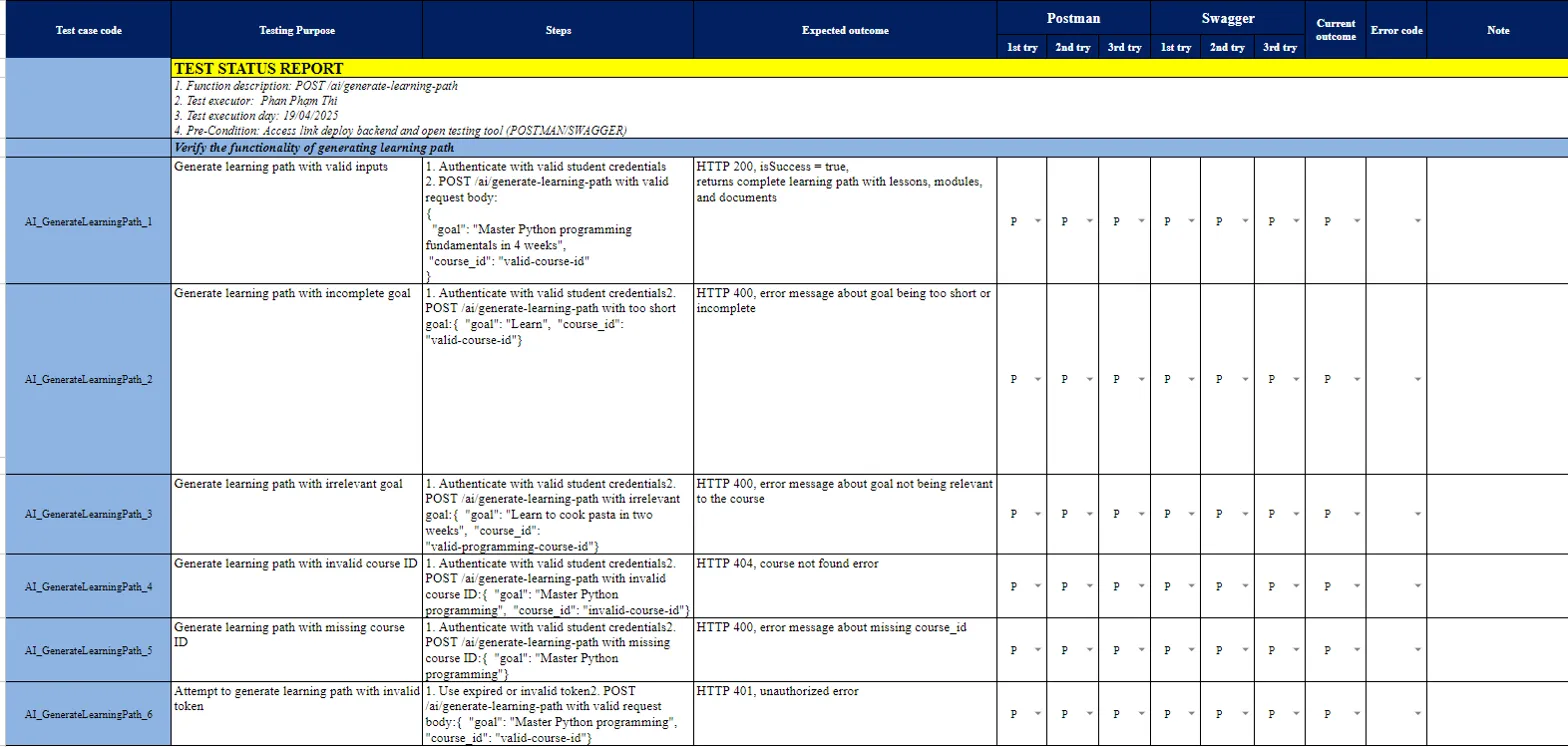
\includegraphics[width=0.8\linewidth]{images/test/test_S1G13.png}
	\caption{Kiểm thử API tạo lộ trình học tập}
	\label{fig:testing_learning_path}
\end{figure}
API \texttt{generate-learning-path} có nhiệm vụ tạo lộ trình học tập dựa trên mục tiêu của sinh viên và khóa học. Các test case kiểm tra nhiều tình huống như:
\begin{itemize}
    \item Tạo lộ trình với dữ liệu hợp lệ (mục tiêu rõ ràng, ID khóa học chính xác)
    \item Tạo lộ trình với mục tiêu không đầy đủ
    \item Tạo lộ trình với mục tiêu không liên quan đến khóa học
    \item Tạo lộ trình với ID khóa học không hợp lệ hoặc thiếu
    \item Xác thực token không hợp lệ
\end{itemize}

Kết quả kiểm thử cho thấy các test case đều vượt qua, với phản hồi thích hợp cho các trường hợp lỗi như mục tiêu không đủ thông tin (HTTP 400), khóa học không tồn tại (HTTP 404), hoặc token không hợp lệ (HTTP 401).

\subsubsection{Kiểm thử API Theo Dõi Tiến Độ Học Tập}
\begin{figure}[H]
	\centering
	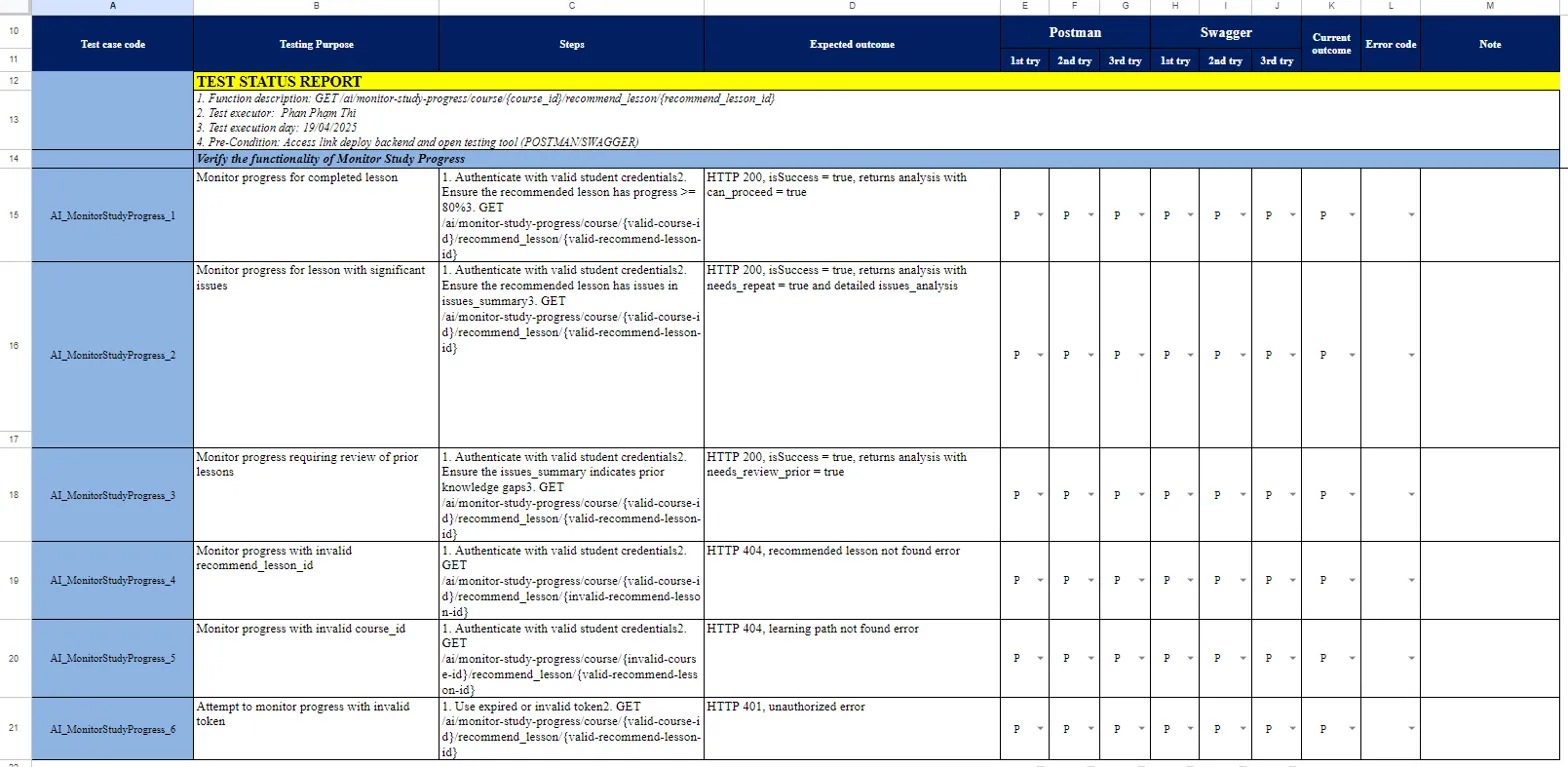
\includegraphics[width=0.8\linewidth]{images/test/test_S1G14.png}
	\caption{Kiểm thử API theo dõi tiến độ học tập}
	\label{fig:testing_tracking_progress}
\end{figure}
API \texttt{monitor-study-progress} được sử dụng để theo dõi tiến độ học tập của sinh viên trong một bài học được đề xuất. Các test case bao gồm:
\begin{itemize}
    \item Theo dõi tiến độ của bài học đã hoàn thành (tiến độ $\geq$ 80\%)
    \item Theo dõi tiến độ bài học với các vấn đề đáng chú ý
    \item Theo dõi tiến độ cần xem lại bài học trước đó
    \item Kiểm tra với ID bài học hoặc khóa học không hợp lệ
    \item Kiểm tra xác thực với token không hợp lệ
\end{itemize}

Tất cả các trường hợp kiểm thử đều đã thành công, với phản hồi chính xác theo từng tình huống (kết quả phân tích, thông báo lỗi).

\subsubsection{Kiểm thử API Tạo Bài Quiz}
\begin{figure}[H]
	\centering
	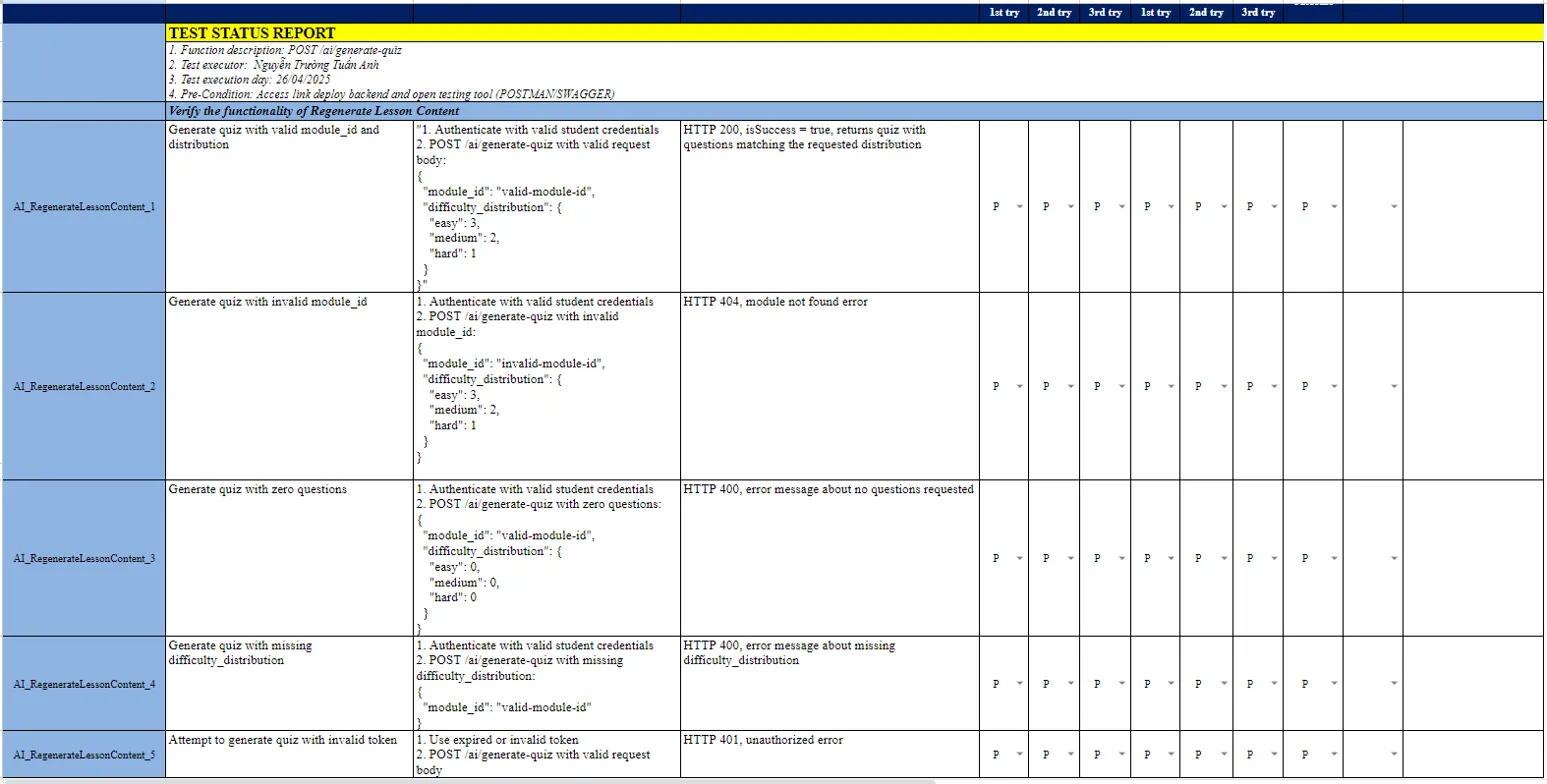
\includegraphics[width=0.8\linewidth]{images/test/test_S1G18.png}
	\caption{Kiểm thử API tạo bài tập quiz}
	\label{fig:testing_quiz}
\end{figure}
API \texttt{generate-quiz} dùng để tạo các bài kiểm tra tự động dựa trên module học tập. Các test case kiểm tra:
\begin{itemize}
    \item Tạo quiz với module\_id hợp lệ và phân bố độ khó hợp lý
    \item Tạo quiz với module\_id không hợp lệ
    \item Tạo quiz với số lượng câu hỏi bằng 0
    \item Tạo quiz thiếu thông tin phân bố độ khó
    \item Xác thực với token không hợp lệ
\end{itemize}

Kết quả kiểm thử cho thấy các phản hồi đều phù hợp với kỳ vọng, bao gồm trả về bài quiz đầy đủ khi dữ liệu hợp lệ và các thông báo lỗi rõ ràng khi dữ liệu không hợp lệ.

\subsubsection{Kiểm thử API Tạo Bài Tập Lập Trình}
\begin{figure}[H]
	\centering
	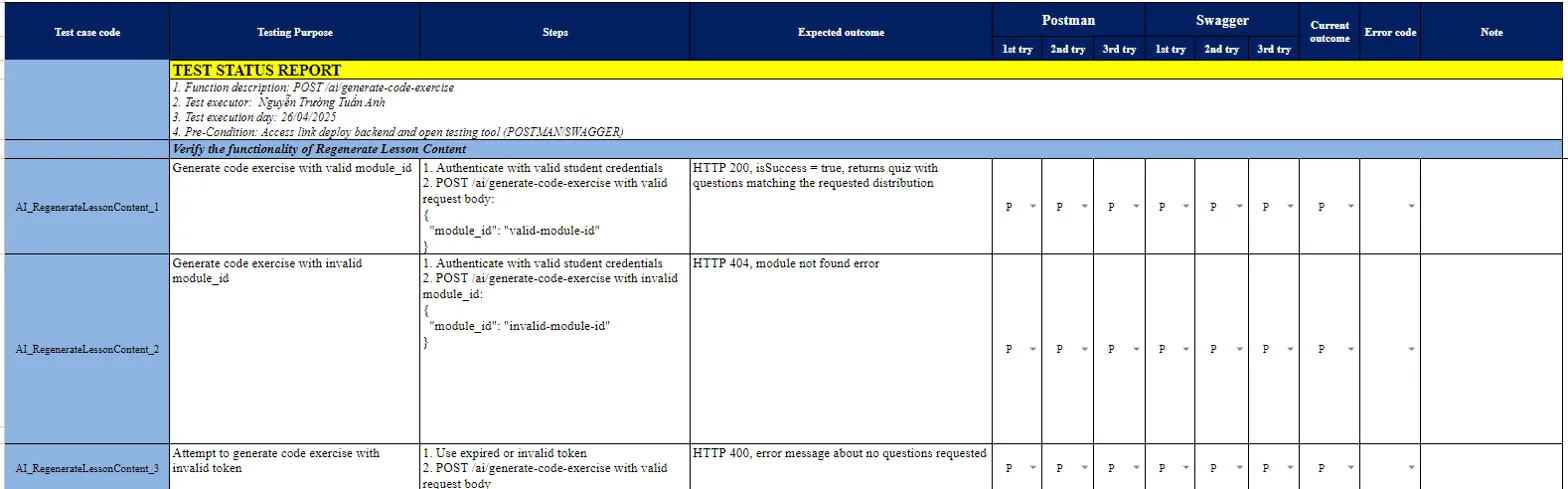
\includegraphics[width=0.8\linewidth]{images/test/test_S1G19.png}
	\caption{Kiểm thử API tạo bài tập code}
	\label{fig:testting_code}
\end{figure}
API \texttt{generate-code-exercise} được sử dụng để tạo bài tập lập trình tự động. Các test case kiểm tra:
\begin{itemize}
    \item Tạo bài tập lập trình với module\_id hợp lệ
    \item Tạo bài tập lập trình với module\_id không hợp lệ
    \item Xác thực với token không hợp lệ
\end{itemize}

Tất cả các test đều thành công, với kết quả trả về phù hợp với yêu cầu và các thông báo lỗi chính xác khi dữ liệu đầu vào không hợp lệ.

\subsubsection{Kiểm thử API Đánh Giá Tiến Độ Học Tập}
\begin{figure}[H]
	\centering
	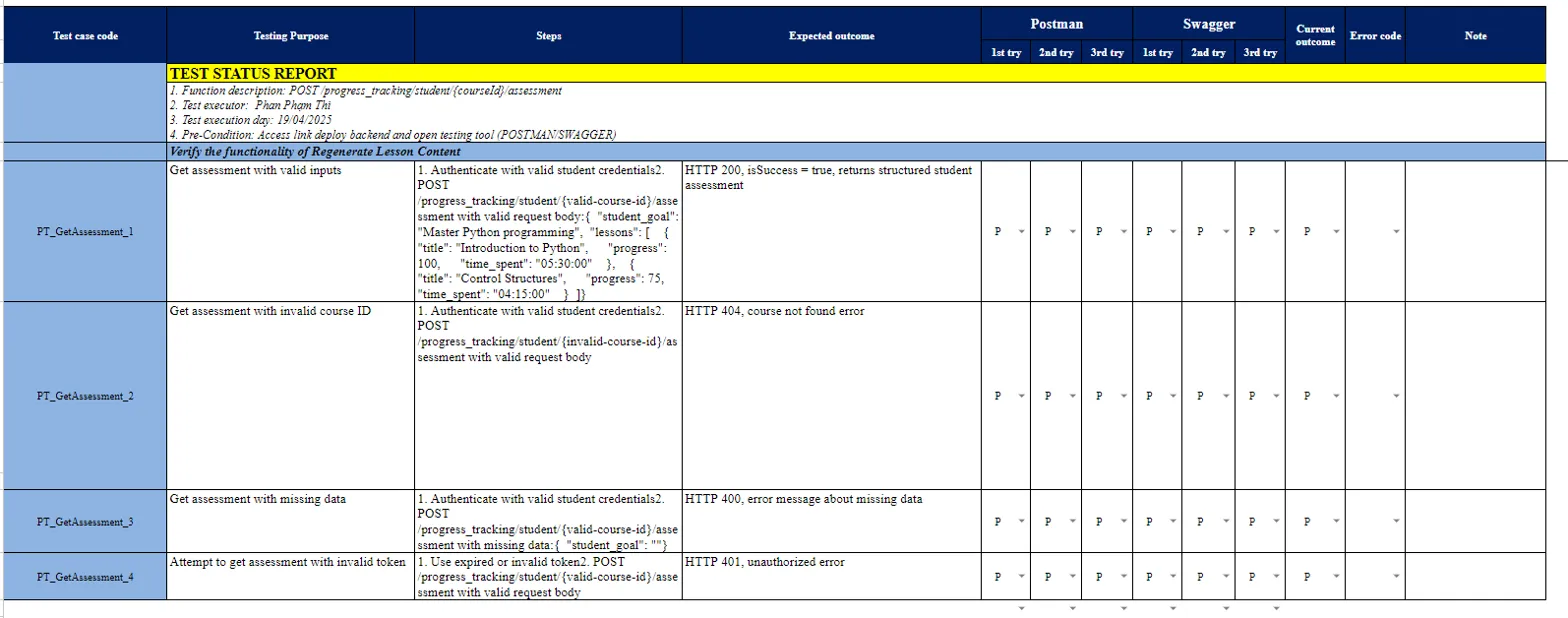
\includegraphics[width=0.8\linewidth]{images/test/test_S1G16.png}
	\caption{Kiểm thử API đánh giá tiến độ học tập}
	\label{fig:testting_evaluation}
\end{figure}
API \texttt{progress\_tracking/student/\{courseId\}/assessment} dùng để tạo đánh giá tiến độ học tập của sinh viên. Các test case kiểm tra:
\begin{itemize}
    \item Lấy đánh giá với dữ liệu đầu vào hợp lệ
    \item Lấy đánh giá với ID khóa học không hợp lệ
    \item Lấy đánh giá với dữ liệu bị thiếu
    \item Xác thực với token không hợp lệ
\end{itemize}

Kết quả kiểm thử cho thấy API phản hồi chính xác với đánh giá có cấu trúc rõ ràng khi dữ liệu hợp lệ, và các thông báo lỗi phù hợp trong các trường hợp khác.

\section{Kết quả kiểm thử API}
\subsection{Kết quả tổng hợp của các testcase}
\begin{figure}[H]
    \centering
    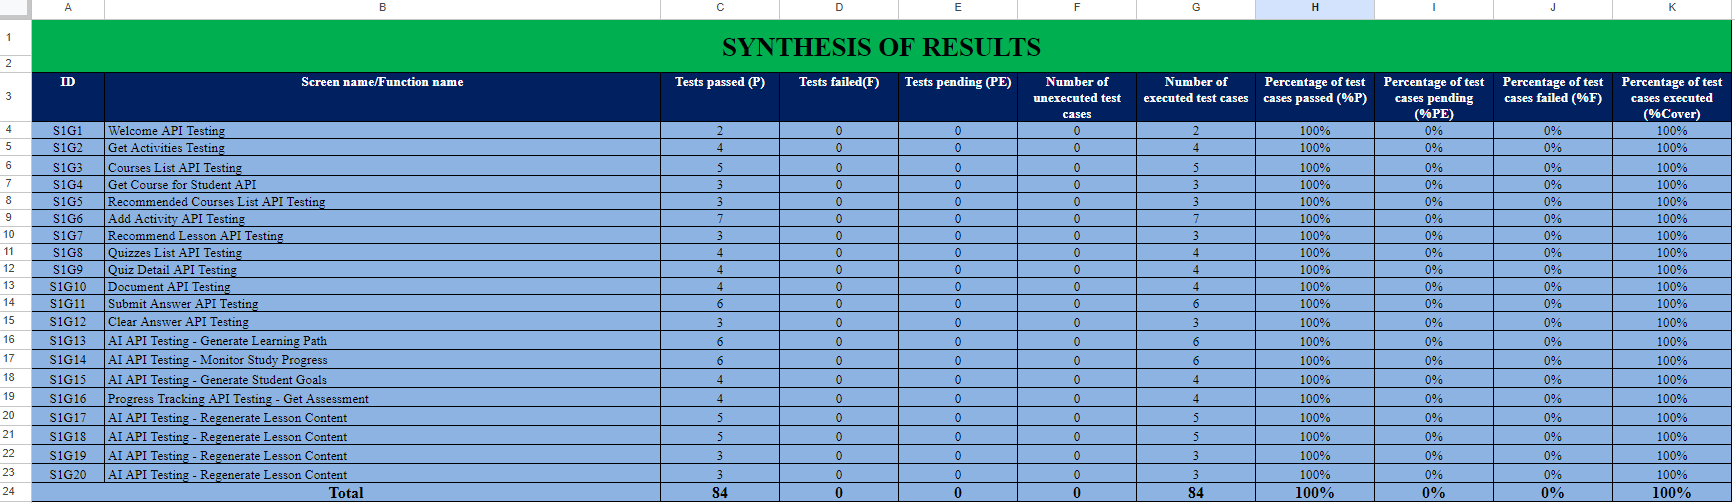
\includegraphics[width=0.8\textwidth]{Images/test/test_summary.png}
    \caption{Kết quả tổng hợp của các testcase}
\end{figure}

\par \textbf{Link QC:} \textcolor{blue}{\href{https://docs.google.com/spreadsheets/d/18kxb6KiawU2gpdIucJwOxST4YF0WvIga/edit?usp=sharing&ouid=101371782687204831060&rtpof=true&sd=true}{QC\_Testcase}}

Bảng tổng hợp kết quả kiểm thử hiển thị kết quả của 20 loại API khác nhau với tổng cộng 84 test case. Phân tích kết quả cho thấy:

\begin{itemize}
    \item \textbf{Số lượng test case đã thực thi:} Toàn bộ 84 test case đã được thực thi, đạt tỷ lệ bao phủ kiểm thử là 100\%.
    \item \textbf{Số lượng test case đã vượt qua:} Tất cả 84 test case (100\%) đều đã vượt qua, chứng tỏ các API đều hoạt động chính xác theo mong đợi.
    \item \textbf{Số lượng test case thất bại:} Không có test case nào thất bại (0\%).
    \item \textbf{Số lượng test case đang chờ xử lý:} Không có test case nào đang chờ xử lý (0\%).
\end{itemize}

Kết quả này chứng tỏ hệ thống hiện đã đạt độ ổn định cao, với tất cả các API đều hoạt động đúng với yêu cầu thiết kế. Cụ thể:

\begin{itemize}
    \item Các API cơ bản như Welcome API, Activities, Courses List và Document API đều hoạt động ổn định.
    \item Các API liên quan đến AI như Generate Learning Path, Monitor Study Progress, Generate Student Goals và Regenerate Lesson Content cũng hoạt động chính xác theo thiết kế, mặc dù đây là những API có độ phức tạp cao hơn.
    \item API xử lý bài tập và kiểm tra (Quiz Detail, Submit Answer) cũng đạt hiệu suất 100\%, đảm bảo tính năng đánh giá học tập hoạt động chính xác.
\end{itemize}
